\documentclass[12pt,a4paper]{article}
\usepackage{graphicx}
\usepackage{geometry}
\usepackage{booktabs}
\usepackage{cite}
\usepackage{amsmath,amssymb}
\usepackage{hyperref}
\geometry{a4paper, margin=1in}

\begin{document}

\begin{titlepage}
    \centering
    
    \vspace*{1cm}
    
    \Large
    \textbf{B.Sc in Computer Science and Engineering Thesis Report on}
    
    \vspace{1.5cm}
    
    \Huge
    \textbf{Poly-Dialectal Neural Machine Translation System for Bangla Regional Dialects}
    
    \vspace{2cm}
    
    \Large
    \textbf{Submitted By}\\
    \vspace{0.5cm}
    \large
    \textbf{Rakib Ullah} \\
    Reg No: 2020331520 \\
    \vspace{0.3cm}
    \textbf{Ruhul Islam Rahul} \\
    Reg No: 2020331529 \\
    \vspace{0.3cm}
    \textbf{Tanbir Ahmed} \\
    Reg No: 2020331516 \\
    
    \vspace{2cm}
    
    \Large
    \textbf{Supervised By}\\
    \vspace{0.5cm}
    \large
    \textbf{Nayan Kumar Nath} \\
    Lecturer \\
    Department of Computer Science and Engineering, \\
    Sylhet Engineering College \\
    
    \vfill
    
    \Large
    \textbf{Department of Computer Science and Engineering}\\
    \vspace{0.2cm}
    \LARGE
    \textbf{SYLHET ENGINEERING COLLEGE, SYLHET}\\
    \vspace{0.5cm}
    \large
    Affiliated with\\
    \Large
    \textbf{Shahjalal University of Science and Technology}\\
    \large
    Sylhet, Bangladesh.\\
    \vspace{0.8cm}
    \large
    22 August, 2026
    
\end{titlepage}

\newpage

\section{Introduction}

\subsection{Background and Motivation}
Bangla (Bengali), an Indo-Aryan language, stands as one of the most widely spoken languages globally, boasting over 240 million native speakers primarily distributed across Bangladesh and the Indian states of West Bengal, Tripura, and Assam. Despite its immense socio-linguistic prominence and rich literary heritage, Bangla is not a monolithic entity; rather, it exhibits substantial intra-language diversity through a vast array of distinct regional dialects. Dialects such as Sylheti, Chittagonian, Barisali, Noakhali, Rangpuri, Rajshahi, and Mymensingh differ markedly from Standard Colloquial Bangla (SCB) across multiple linguistic strata. These divergences manifest as profound phonological variations, complex morphological inflections, altered syntactic structures, and highly localized lexical choices. In extreme cases, such as the Chittagonian or Sylheti dialects, the linguistic deviation is so severe that they are often bordering on mutual unintelligibility with Standard Bangla.

This deep intra-language divergence engenders significant communication barriers within the broader socio-economic framework. Native speakers of peripheral regional dialects frequently encounter difficulties in seamless communication with speakers of other dialects, as well as in formal interactions, legal proceedings, and educational instructions traditionally conducted in Standard Bangla. Furthermore, modern Natural Language Processing (NLP) tools, machine translation systems, and digital interfaces---ranging from virtual assistants to automated governance platforms---are overwhelmingly optimized exclusively for Standard Bangla. Consequently, millions of dialectal speakers face systemic digital marginalization and language-access inequality, lacking automated communication technologies tuned to their native spoken forms. This technological disparity highlights an urgent need for inclusive NLP systems that can bridge the communication gap without enforcing linguistic homogenization.

\subsection{Problem Statement}
In recent years, Neural Machine Translation (NMT) architectures and Large Language Models (LLMs) have achieved state-of-the-art results for cross-lingual tasks involving high-resource languages. However, their efficacy degrades severely when applied to low-resource intra-language dialectal shifts. Most existing Bangla NLP benchmarks and pre-trained models treat the language as a singular, uniform distribution, fundamentally ignoring the complex cross-dialectal matrix. 

This oversight stems from a confluence of critical technical challenges. Firstly, there is an acute scarcity of multi-dialectal parallel corpora required to effectively fine-tune deep neural networks. Secondly, the lack of standardized orthography for regional dialects exacerbates tokenization mismatches; standard Byte-Pair Encoding (BPE) or WordPiece algorithms optimized for SCB frequently fragment dialectal words into meaningless subwords, destroying semantic integrity. Finally, existing regional text datasets suffer from severe class imbalance and are predominantly tailored for simple classification tasks rather than complex generative alignment. Addressing these challenges requires a paradigm shift from uni-dialectal modeling to a holistic, poly-dialectal approach.

\subsection{Proposed System and Contributions}
To address these fundamental limitations, this research introduces a unified \textbf{Poly-Dialectal Neural Machine Translation System} tailored specifically for the morphological and syntactic nuances of Bangla regional dialects. As illustrated in Figure~\ref{fig:overview}, our architecture enables robust, multi-directional translation across three core operational paradigms: Dialect $\rightarrow$ Standard Bangla, Standard Bangla $\rightarrow$ Dialect, and direct Dialect $\rightarrow$ Dialect translation, thereby eliminating the cascading errors typically introduced by pivot-based translation methods.

\begin{figure}[htbp]
  \centering
  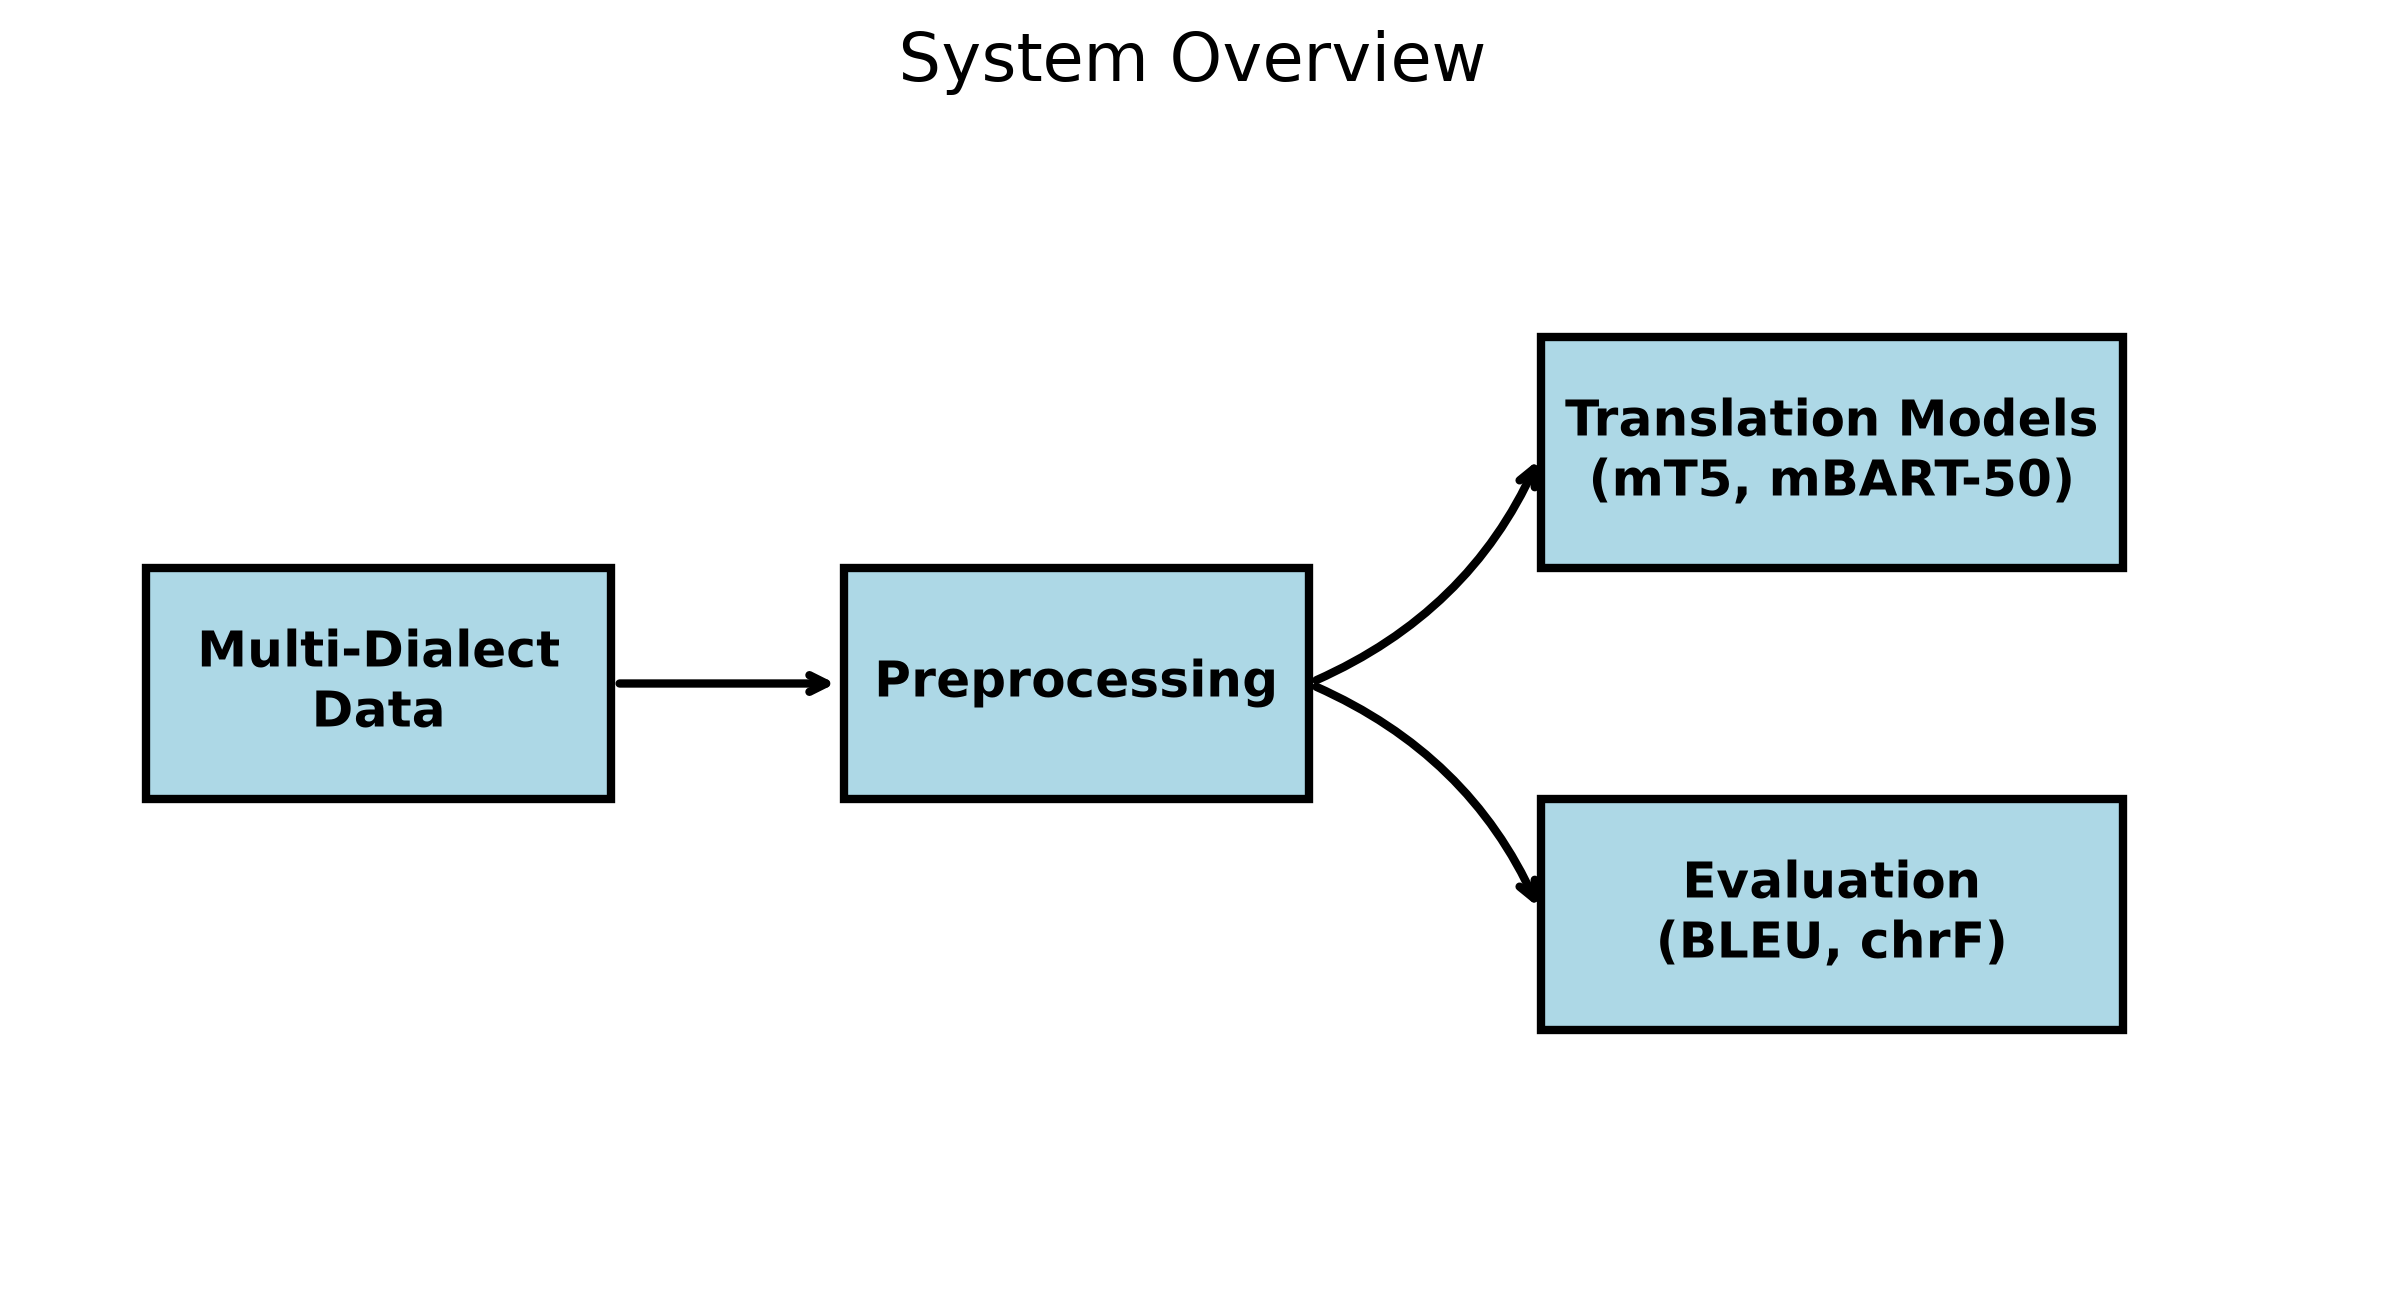
\includegraphics[width=0.85\textwidth]{graphics/overview.png}
  \caption{High-level architectural workflow of the Poly-Dialectal Neural Machine Translation Framework, depicting data alignment, model fine-tuning, and multi-directional evaluation.}
  \label{fig:overview}
\end{figure}

The primary contributions of this thesis are summarized as follows:
\begin{enumerate}
    \item \textbf{Largest Multi-Dialectal Parallel Corpus:} We construct the most expansive multi-dialect machine translation corpus for Bangla to date, compiling 31,460 Standard Bengali sentences paired intricately across 8 major regional dialects (including Sylheti, Chittagonian, Barisali, Noakhali, Rangpuri, Rajshahi, and Mymensingh). This extensive curation yields a grand total of over 100,000 parallel sentence pairs, meticulously aligned to capture nuanced dialectal variations.
    \item \textbf{Comprehensive Evaluation of Multilingual NMT Architectures:} We systematically fine-tune and empirically evaluate prominent Sequence-to-Sequence models---specifically mT5, mBART-50, NLLB-200, and BanglaT5---under diverse, multi-directional translation settings. 
    \item \textbf{Systematic Cross-Dialectal Linguistic Analysis:} We conduct a rigorous quantitative characterization of cross-dialectal transfer mechanisms. By analyzing performance metrics (BLEU, chrF++, TER, METEOR) against linguistic divergences, we uncover how morphological proximity influences neural machine translation efficacy.
\end{enumerate}

\subsection{Thesis Organization}
The remainder of this report is organized as follows: Section 2 critically reviews related literature on Bangla regional NLP and dialectal machine translation. Section 3 presents our research hypothesis and main objectives. Section 4 details the methodology, dataset alignment strategies, and architectural model configurations. Section 5 presents a comprehensive evaluation of the experimental results. Finally, Section 6 discusses the limitations of the current framework and proposes future research directions, followed by concluding remarks in Section 7.

\newpage

\section{Literature Review}

\subsection{Overview of Regional Bangla NLP}
Historically, the development of linguistic resources for Bangla has heavily favored Standard Colloquial Bangla, leaving regional dialects severely underrepresented in the NLP ecosystem. However, over the past few years, interest in low-resource regional Bangla NLP has seen a significant upsurge. Initial studies focused predominantly on resource creation for text classification and sentiment analysis tasks for specific regions. 

Sultana et al.~\cite{sultana2024bdregion} established the \textit{BdRegionText} corpus, a pioneering effort for regional text classification, which starkly demonstrated the performance bottleneck of standard classifiers when exposed to rich dialectal vocabulary. Building on the need for broader representation, Mahi et al.~\cite{mahi2025bangladial} released \textit{BanglaDial}, a merged text dataset that brought to light the severe class imbalance issues and data scarcity prevalent across different regional dialects.

In specialized downstream NLP tasks, the complexity of dialectal morphology continues to pose significant hurdles. Kundu et al.~\cite{kundu2026anubhuti} introduced \textit{ANUBHUTI}, a dedicated corpus targeting sentiment analysis in regional languages, revealing that emotion markers vary significantly across regional boundaries. For the crucial task of offensive speech identification, Fayaz et al.~\cite{fayaz2025bidwesh} developed \textit{BIDWESH}, evaluating hate speech detection mechanisms across regional dialects and proving that SCB-trained toxicity classifiers fail to generalize to dialectal slang. Concurrently, Paul et al.~\cite{paul2025ancholik} formulated \textit{ANCHOLIK-NER}, providing essential named entity annotations across regional variants to facilitate information extraction in non-standard texts.

\subsection{Dialectal Machine Translation and LLM Benchmarks}
While text classification laid the groundwork, direct efforts in generative machine translation for Bangla dialects have emerged only recently, driven by the advent of massively multilingual neural models. Early translation corpora were highly localized. For instance, Chowdhury et al.~\cite{chowdhury2025chatgaiyya} built \textit{ChatgaiyyaAlap}, a dedicated parallel corpus strictly designed for translating Chittagonian dialect sentences to Standard Bangla. To expand the dialectal scope, Sultana et al.~\cite{sultana2025onubad} presented \textit{ONUBAD}, providing an initial generalized resource for automated regional dialect conversion. This was followed by Faria et al.~\cite{faria2025vashantor}, who introduced \textit{Vashantor}, a multilingual benchmark covering five regional dialects. Though a significant step forward, \textit{Vashantor} remained constrained by its limited volume, offering only 2,500 sentences per dialect.

More recently, the research community has pivoted towards exploring the zero-shot and few-shot capabilities of Large Language Models (LLMs) for dialect translation. Mahjabin et al.~\cite{mahjabin2025banglachq} constructed \textit{BanglaCHQ-Prantik} to benchmark state-of-the-art LLMs against human-evaluated dialect translation standards. Similarly, Jawad et al.~\cite{jawad2025dialtsa} presented \textit{DIALTSA-BN}, evaluating LLM capabilities in joint dialect translation and sentiment analysis. Furthermore, Bhuiyan et al.~\cite{bhuiyan2025bhasabodh} explored \textit{BhasaBodh}, investigating methods to bridge Bangla dialects and romanized forms through advanced machine translation techniques. Despite these advancements, fine-tuned NMT models consistently outperform generalized LLMs in specialized low-resource dialectal translation due to the LLMs' inherent lack of dialect-specific pre-training data.

\subsection{Critical Synthesis and Research Gap}
While the aforementioned contributions have collectively laid a valuable foundation for Bangla dialectal NLP, a critical review reveals several major structural and methodological shortcomings that currently stifle the development of robust, production-ready translation systems:

\begin{enumerate}
    \item \textbf{Single-Dialect Isolation:} Corpora such as \textit{ChatgaiyyaAlap} focus exclusively on a single dialect pair (e.g., Chittagonian-Standard). Models trained on such isolated datasets fail entirely to generalize across other regional dialects, necessitating the training of separate, disjoint models for every region.
    \item \textbf{Severe Corpus Volume Limitations:} Multi-dialect datasets like \textit{Vashantor} offer only modest data volumes (e.g., 2,500 samples per dialect). This limited scale is vastly insufficient for the deep fine-tuning required by large sequence-to-sequence neural architectures like mT5 or mBART-50, inevitably leading to overfitting and poor generalization on unseen data.
    \item \textbf{The Pivot Translation Problem:} Existing works lack a unified framework capable of translating directly between different regional dialects (e.g., Sylheti $\rightarrow$ Chittagonian). Current systems force a ``pivot'' approach, routing translation through Standard Bangla as an intermediary (Sylheti $\rightarrow$ SCB $\rightarrow$ Chittagonian). This two-step process compounds translation errors, degrading the final semantic accuracy and fluency.
\end{enumerate}

To definitively resolve these limitations, our work introduces a comprehensive, balanced, poly-dialectal parallel corpus that is orders of magnitude larger than previous efforts. By fine-tuning state-of-the-art Transformer models on this expansive dataset, we enable direct, multi-directional, poly-dialectal translation within a single, unified neural architecture.

\bibliographystyle{plain}
\bibliography{biblography}

\end{document}
